%%%%%%%%%%%%%%%%%%%%%%%%%%%%%%%%%%%%%%%%
% datoteka diploma-vzorec.tex
%
% vzorčna datoteka za pisanje diplomskega dela v formatu LaTeX
% na UL Fakulteti za računalništvo in informatiko
%
% vkup spravil Gašper Fijavž, december 2010
% 
%
%
% verzija 12. februar 2014 (besedilo teme, seznam kratic, popravki Gašper Fijavž)
% verzija 10. marec 2014 (redakcijski popravki Zoran Bosnić)
% verzija 11. marec 2014 (redakcijski popravki Gašper Fijavž)
% verzija 15. april 2014 (pdf/a 1b compliance, not really - just claiming, Damjan Cvetan, Gašper Fijavž)
% verzija 23. april 2014 (privzeto cc licenca)
% verzija 16. september 2014 (odmiki strain od roba)
% verzija 28. oktober 2014 (odstranil vpisno številko)
% verija 5. februar 2015 (Literatura v kazalu, online literatura)
% verzija 25. september 2015 (angl. naslov v izjavi o avtorstvu)
% verzija 26. februar 2016 (UL izjava o avtorstvu)
% verzija 16. april 2016 (odstranjena izjava o avtorstvu)
% verzija 5. junij 2016 (Franc Solina dodal vrstice, ki jih je označil s svojim imenom)


\documentclass[a4paper, 12pt]{book}
%\documentclass[a4paper, 12pt, draft]{book}  Nalogo preverite tudi z opcijo draft, ki vam bo pokazala, katere vrstice so predolge!



\usepackage[utf8x]{inputenc}   % omogoča uporabo slovenskih črk kodiranih v formatu UTF-8
\usepackage[slovene,english]{babel}    % naloži, med drugim, slovenske delilne vzorce
\usepackage[pdftex]{graphicx}  % omogoča vlaganje slik različnih formatov
\usepackage{fancyhdr}          % poskrbi, na primer, za glave strani
\usepackage{amssymb}           % dodatni simboli
\usepackage{amsmath}           % eqref, npr.
%\usepackage{hyperxmp}
\usepackage[hyphens]{url}  % dodal Solina
\usepackage{comment}       % dodal Solina

\usepackage[pdftex, colorlinks=true,
						citecolor=black, filecolor=black, 
						linkcolor=black, urlcolor=black,
						pagebackref=false, 
						pdfproducer={LaTeX}, pdfcreator={LaTeX}, hidelinks]{hyperref}

\usepackage{color}       % dodal Solina
\usepackage{soul}       % dodal Solina

%%%%%%%%%%%%%%%%%%%%%%%%%%%%%%%%%%%%%%%%
%	DIPLOMA INFO
%%%%%%%%%%%%%%%%%%%%%%%%%%%%%%%%%%%%%%%%
\newcommand{\ttitle}{Digitalni video efekti za After Effects}
\newcommand{\ttitleEn}{Digital video effects for After Effects}
\newcommand{\tsubject}{\ttitle}
\newcommand{\tsubjectEn}{\ttitleEn}
\newcommand{\tauthor}{Maj Smerkol}
\newcommand{\tkeywords}{video, After Effects, vizualni učinki, posebni učinki}
\newcommand{\tkeywordsEn}{video, After Effects, visual effects, special effects}


%%%%%%%%%%%%%%%%%%%%%%%%%%%%%%%%%%%%%%%%
%	HYPERREF SETUP
%%%%%%%%%%%%%%%%%%%%%%%%%%%%%%%%%%%%%%%%
\hypersetup{pdftitle={\ttitle}}
\hypersetup{pdfsubject=\ttitleEn}
\hypersetup{pdfauthor={\tauthor, ms5013@student.uni-lj.si}}
\hypersetup{pdfkeywords=\tkeywordsEn}


 


%%%%%%%%%%%%%%%%%%%%%%%%%%%%%%%%%%%%%%%%
% postavitev strani
%%%%%%%%%%%%%%%%%%%%%%%%%%%%%%%%%%%%%%%%  

\addtolength{\marginparwidth}{-20pt} % robovi za tisk
\addtolength{\oddsidemargin}{40pt}
\addtolength{\evensidemargin}{-40pt}

\renewcommand{\baselinestretch}{1.3} % ustrezen razmik med vrsticami
\setlength{\headheight}{15pt}        % potreben prostor na vrhu
\renewcommand{\chaptermark}[1]%
{\markboth{\MakeUppercase{\thechapter.\ #1}}{}} \renewcommand{\sectionmark}[1]%
{\markright{\MakeUppercase{\thesection.\ #1}}} \renewcommand{\headrulewidth}{0.5pt} \renewcommand{\footrulewidth}{0pt}
\fancyhf{}
\fancyhead[LE,RO]{\sl \thepage} 
%\fancyhead[LO]{\sl \rightmark} \fancyhead[RE]{\sl \leftmark}
\fancyhead[RE]{\sc \tauthor}              % dodal Solina
\fancyhead[LO]{\sc Diplomska naloga}     % dodal Solina


\newcommand{\BibTeX}{{\sc Bib}\TeX}

%%%%%%%%%%%%%%%%%%%%%%%%%%%%%%%%%%%%%%%%
% naslovi
%%%%%%%%%%%%%%%%%%%%%%%%%%%%%%%%%%%%%%%%  


\newcommand{\autfont}{\Large}
\newcommand{\titfont}{\LARGE\bf}
\newcommand{\clearemptydoublepage}{\newpage{\pagestyle{empty}\cleardoublepage}}
\setcounter{tocdepth}{1}	      % globina kazala

%%%%%%%%%%%%%%%%%%%%%%%%%%%%%%%%%%%%%%%%
% konstrukti
%%%%%%%%%%%%%%%%%%%%%%%%%%%%%%%%%%%%%%%%  
\newtheorem{izrek}{Izrek}[chapter]
\newtheorem{trditev}{Trditev}[izrek]
\newenvironment{dokaz}{\emph{Dokaz.}\ }{\hspace{\fill}{$\Box$}}

%%%%%%%%%%%%%%%%%%%%%%%%%%%%%%%%%%%%%%%%%%%%%%%%%%%%%%%%%%%%%%%%%%%%%%%%%%%%%%%
%% PDF-A
%%%%%%%%%%%%%%%%%%%%%%%%%%%%%%%%%%%%%%%%%%%%%%%%%%%%%%%%%%%%%%%%%%%%%%%%%%%%%%%


%%%%%%%%%%%%%%%%%%%%%%%%%%%%%%%%%%%%%%%% 
% define medatata
%%%%%%%%%%%%%%%%%%%%%%%%%%%%%%%%%%%%%%%% 
\def\Title{\ttitle}
\def\Author{\tauthor, matjaz.kralj@fri.uni-lj.si}
\def\Subject{\ttitleEn}
\def\Keywords{\tkeywordsEn}

%%%%%%%%%%%%%%%%%%%%%%%%%%%%%%%%%%%%%%%% 
% \convertDate converts D:20080419103507+02'00' to 2008-04-19T10:35:07+02:00
%%%%%%%%%%%%%%%%%%%%%%%%%%%%%%%%%%%%%%%% 
\def\convertDate{%
    \getYear
}

{\catcode`\D=12
 \gdef\getYear D:#1#2#3#4{\edef\xYear{#1#2#3#4}\getMonth}
}
\def\getMonth#1#2{\edef\xMonth{#1#2}\getDay}
\def\getDay#1#2{\edef\xDay{#1#2}\getHour}
\def\getHour#1#2{\edef\xHour{#1#2}\getMin}
\def\getMin#1#2{\edef\xMin{#1#2}\getSec}
\def\getSec#1#2{\edef\xSec{#1#2}\getTZh}
\def\getTZh +#1#2{\edef\xTZh{#1#2}\getTZm}
\def\getTZm '#1#2'{%
    \edef\xTZm{#1#2}%
    \edef\convDate{\xYear-\xMonth-\xDay T\xHour:\xMin:\xSec+\xTZh:\xTZm}%
}

\expandafter\convertDate\pdfcreationdate 

%%%%%%%%%%%%%%%%%%%%%%%%%%%%%%%%%%%%%%%%
% get pdftex version string
%%%%%%%%%%%%%%%%%%%%%%%%%%%%%%%%%%%%%%%% 
\newcount\countA
\countA=\pdftexversion
\advance \countA by -100
\def\pdftexVersionStr{pdfTeX-1.\the\countA.\pdftexrevision}


%%%%%%%%%%%%%%%%%%%%%%%%%%%%%%%%%%%%%%%%
% XMP data
%%%%%%%%%%%%%%%%%%%%%%%%%%%%%%%%%%%%%%%%  
\usepackage{xmpincl}
\includexmp{pdfa-1b}

%%%%%%%%%%%%%%%%%%%%%%%%%%%%%%%%%%%%%%%%
% pdfInfo
%%%%%%%%%%%%%%%%%%%%%%%%%%%%%%%%%%%%%%%%  
\pdfinfo{%
    /Title    (\ttitle)
    /Author   (\tauthor, damjan@cvetan.si)
    /Subject  (\ttitleEn)
    /Keywords (\tkeywordsEn)
    /ModDate  (\pdfcreationdate)
    /Trapped  /False
}


%%%%%%%%%%%%%%%%%%%%%%%%%%%%%%%%%%%%%%%%%%%%%%%%%%%%%%%%%%%%%%%%%%%%%%%%%%%%%%%
%%%%%%%%%%%%%%%%%%%%%%%%%%%%%%%%%%%%%%%%%%%%%%%%%%%%%%%%%%%%%%%%%%%%%%%%%%%%%%%

\begin{document}
\selectlanguage{slovene}
\frontmatter
\setcounter{page}{1} %
\renewcommand{\thepage}{}       % preprecimo težave s številkami strani v kazalu
\newcommand{\sn}[1]{"`#1"'}                    % dodal Solina (slovenski narekovaji)

%%%%%%%%%%%%%%%%%%%%%%%%%%%%%%%%%%%%%%%%
%naslovnica
 \thispagestyle{empty}%
   \begin{center}
    {\large\sc Univerza v Ljubljani\\%
      Fakulteta za računalništvo in informatiko}%
    \vskip 10em%
    {\autfont \tauthor\par}%
    {\titfont \ttitle \par}%
    {\vskip 3em \textsc{DIPLOMSKO DELO\\[5mm]         % dodal Solina za ostale študijske programe
%    VISOKOŠOLSKI STROKOVNI ŠTUDIJSKI PROGRAM\\ PRVE STOPNJE\\ RAČUNALNIŠTVO IN INFORMATIKA}\par}%
    UNIVERZITETNI  ŠTUDIJSKI PROGRAM\\ PRVE STOPNJE\\ RAČUNALNIŠTVO IN INFORMATIKA}\par}%
%    INTERDISCIPLINARNI UNIVERZITETNI\\ ŠTUDIJSKI PROGRAM PRVE STOPNJE\\ RAČUNALNIŠTVO IN MATEMATIKA}\par}%
%    INTERDISCIPLINARNI UNIVERZITETNI\\ ŠTUDIJSKI PROGRAM PRVE STOPNJE\\ UPRAVNA INFORMATIKA}\par}%
%    INTERDISCIPLINARNI UNIVERZITETNI\\ ŠTUDIJSKI PROGRAM PRVE STOPNJE\\ MULTIMEDIJA}\par}%
    \vfill\null%
    {\large \textsc{Mentor}: doc.\ dr.  Narvika Bovcon\par}%
%   {\large \textsc{Somentor}:  izr.\ prof.\ dr. Martin Krpan \par}%
    {\vskip 2em \large Ljubljana, 2017 \par}%
\end{center}
% prazna stran
%\clearemptydoublepage      % dodal Solina (izjava o licencah itd. se izpiše na hrbtni strani naslovnice)

%%%%%%%%%%%%%%%%%%%%%%%%%%%%%%%%%%%%%%%%
%copyright stran
\thispagestyle{empty}
\vspace*{8cm}

\noindent
{\sc Copyright}. 
Rezultati diplomske naloge so intelektualna lastnina avtorja in Fakultete za računalništvo in informatiko Univerze v Ljubljani.
Za objavo in koriščenje rezultatov diplomske naloge je potrebno pisno privoljenje avtorja, Fakultete za računalništvo in informatiko ter mentorja.

\begin{center}
\mbox{}\vfill
\emph{Besedilo je oblikovano z urejevalnikom besedil \LaTeX.}
\end{center}
% prazna stran
\clearemptydoublepage

%%%%%%%%%%%%%%%%%%%%%%%%%%%%%%%%%%%%%%%%
% stran 3 med uvodnimi listi
\thispagestyle{empty}
\vspace*{4cm}

\noindent
Fakulteta za računalništvo in informatiko izdaja naslednjo nalogo:
\medskip
\begin{tabbing}
\hspace{32mm}\= \hspace{6cm} \= \kill


Tematika naloge:
\end{tabbing}
Besedilo teme diplomskega dela študent prepiše iz študijskega informacijskega sistema, kamor ga je vnesel mentor. V nekaj stavkih bo opisal, kaj pričakuje od kandidatovega diplomskega dela. Kaj so cilji, kakšne metode uporabiti, morda bo zapisal tudi ključno literaturo.
\vspace{15mm}




\vspace{2cm}

% prazna stran
\clearemptydoublepage

% zahvala
\thispagestyle{empty}\mbox{}\vfill\null\it%
\noindent
Na tem mestu zapišite, komu se zahvaljujete za izdelavo diplomske naloge. Pazite, da ne boste koga pozabili. Utegnil vam bo zameriti. Temu se da izogniti tako, da celotno zahvalo izpustite.
\rm\normalfont

% prazna stran
\clearemptydoublepage

%%%%%%%%%%%%%%%%%%%%%%%%%%%%%%%%%%%%%%%%
% posvetilo, če sama zahvala ne zadošča :-)
\thispagestyle{empty}\mbox{}{\vskip0.20\textheight}\mbox{}\hfill\begin{minipage}{0.55\textwidth}%
Svoji dragi Alenčici.
\normalfont\end{minipage}

% prazna stran
\clearemptydoublepage


%%%%%%%%%%%%%%%%%%%%%%%%%%%%%%%%%%%%%%%%
% kazalo
\pagestyle{empty}
\def\thepage{}% preprecimo tezave s stevilkami strani v kazalu
\tableofcontents{}


% prazna stran
\clearemptydoublepage

%%%%%%%%%%%%%%%%%%%%%%%%%%%%%%%%%%%%%%%%
% seznam kratic

\chapter*{Seznam uporabljenih kratic}  % spremenil Solina, da predolge vrstice ne gredo preko desnega roba

\noindent\begin{tabular}{p{0.1\textwidth}|p{.4\textwidth}|p{.4\textwidth}}    % po potrebi razširi prvo kolono tabele na račun drugih dveh!
  {\bf kratica} & {\bf angleško}              				& {\bf slovensko} \\ \hline
  {\bf VFX}      & visual effects               				& vizualni učinki \\
  {\bf SFX}      & special effects              				& posebni učinki \\
  {\bf AEGP}   & After Effects general purpose plug-in 	& splošno namenski vtičnik za After Effects \\
  {\bf AE}       & Adobe After Effects 				&  Adobe After Effects \\
  {\bf SDK}     & software development kit 			&  paket za razvoj programske opreme \\
  {\bf CGI}	& computer generated imagery			& računalniško generirana grafika \\

\end{tabular}


% prazna stran
\clearemptydoublepage

%%%%%%%%%%%%%%%%%%%%%%%%%%%%%%%%%%%%%%%%
% povzetek
\addcontentsline{toc}{chapter}{Povzetek}
\chapter*{Povzetek}

\noindent\textbf{Naslov:} \ttitle
\bigskip

\noindent\textbf{Avtor:} \tauthor
\bigskip

%\noindent\textbf{Povzetek:} 
\noindent V vzorcu je predstavljen postopek priprave diplomskega dela z uporabo okolja \LaTeX. Vaš povzetek mora sicer vsebovati približno 100 besed, ta tukaj je odločno prekratek.
Dober povzetek vključuje: (1) kratek opis obravnavanega problema, (2) kratek opis vašega pristopa za reševanje tega problema in (3) (najbolj uspešen) rezultat ali prispevek magistrske naloge.

\bigskip

\noindent\textbf{Ključne besede:} \tkeywords.
% prazna stran
\clearemptydoublepage

%%%%%%%%%%%%%%%%%%%%%%%%%%%%%%%%%%%%%%%%
% abstract
\selectlanguage{english}
\addcontentsline{toc}{chapter}{Abstract}
\chapter*{Abstract}

\noindent\textbf{Title:} \ttitleEn
\bigskip

\noindent\textbf{Author:} \tauthor
\bigskip

%\noindent\textbf{Abstract:} 
\noindent This sample document presents an approach to typesetting your BSc thesis using \LaTeX. 
A proper abstract should contain around 100 words which makes this one way too short.
\bigskip

\noindent\textbf{Keywords:} \tkeywordsEn.
\selectlanguage{slovene}
% prazna stran
\clearemptydoublepage

%%%%%%%%%%%%%%%%%%%%%%%%%%%%%%%%%%%%%%%%
\mainmatter
\setcounter{page}{1}
\pagestyle{fancy}

\chapter{Uvod}

Cilj diplomske naloge je raziskati metode razvoja vtičnikov za programsko orodje Adobe After Effects (v nadaljevanju AE). 
AE je programski paket, namenjen montaži videa in izdelavi vizualnih efektov. 
Ena izmed njegovih dobrih lastnosti je razširljivost s pomočjo vtičnikov, ki omogočajo dodajanje poljubnih funckionalnosti programskemu paketu. 
Razširjanje je omogočeno prek programskega vmesnika in prosto dostopne razvojne dokumentacije za uporabo le tega. 

Vtičnike za AE lahko delimo v 4 kategorije: 
splošno namenske vtičnike (AEGP), 
vizualne učinke (effect), 
vhodno izhodne vtičnike (IO) in 
vtičnike Artisan, ki prevzamejo upodabljanje 3D slojev oziroma nadomestijo privzeti algoritem za upodabljanje v AE. 
Gostitelj še vedno sam skrbi za upodabljanje 2D slojev. 
Ker sem se odločil za razvoj vizualnih učinkov, je izbira med tipi vtičnikov jasna. 
Vtičniki za vizualne učinke implementirajo VFX kot operacijo nad posameznimi sličicami v videu. 
Programski vmesnik AE ponuja nemalo operacij, ki pospešijo izvajanje operacij nad piksli in skrajšajo čas razvoja, saj ponujajo visokonivojski dostop do vgrajenih funkcij AE. 

Splošno namenski vtičniki zahtevajo več resursov od sistema, na katerem tečejo, omogočajo pa programerju več možnosti itegracije z AE, spreminjanje uporabniškega vmesnika in odzivanje na interno stanje celotnega programskega paketa. 
Omogočajo mnogo več, kot potrebujemo za implementacijo tipičnih vizualnih učinkov. 
Vhodno izhodni vtičniki so namenjeni dodajanju podpore za branje in pisanje novih datotečnih formatov, implementaciji kodekov in podobno.

Pri razvoju VFX je seveda prvi korak ugotavljanje namena vizualnega učinka oziroma definiranje umetniške vizije. 
Pred tem sem pregledal obstoječe vtičnike. 
Po namenu sem jih ločil v tri kategorije. 
Prva kategorija so vtičniki za popravljanje izvornih posnetkov, kot so odstranjevanje šuma, popravljanje raznih vizualnih artefaktov in podobno. 
Namen teh vtičnikov je reševanje slabih posnetkov, kadar ponovni zajem videa oziroma ponovno snemanje ni mogoče, zaradi cene, pomanjkanja časa ali drugih razlogov. 
Le redko lahko s pomočjo teh vtičnikov dosežemo rezultate enake kvalitete, kot če bi bili posnetki dobri. 

V drugo kategorijo štejem efekte, ki so namenjeni dodajanju vrednosti posnetki v post produkciji. 
Večino vizualnih učinkov pravzaprav lahko štejemo v to kategorijo. 
Sem spadajo tudi vsi tisti efekti, ki vizualno pomagajo pripovedništvu, pomagajo ustvariti fiktiven svet, like in podobno. 

V tretjo kategorijo uvrščam destruktivne efekte - to so tisti, ki ne dodajajo informacij sliki, ampak nasprotno zmanjšajo kvaliteto slike za dosego nekega vizualnega sloga ali pa pomagajo ustvarjati vzdušje in gledalcu, če so uspešno uporabljeni, lahko vzbudijo določena čustva. 
Primere takšnih efektov lahko najdemo marsikje, v popularni kulturi (Mr Robot, 2015), %!TODO preveri podatke + slika
računalniških igrah (SOMA, 2016) % !TODO poglej podateke in slika
 in filmih (The Matrix, 1999), % !TODO opklepaj izpolni.
na različne načine proizvedene vizualne artefakte pa celo v galerijah in knjižnih zbirkah umetniških del (ang. {\it ASCII Graphic Glitch Art}, Rozita Fogelman).

 % !TODO zgodovina glitch art IZ KNJIG NOVIH don't translate glitch art
% !TODO medijski jezik, video jezik, kaj pomenijo glitchi danes in mogoče kaj so včasih.


\chapter{Vizualni učinki v filmu in videu}

% !TODO  namen montaže, montaža kot korak postprodukcije, linearna in nelinearna montaža (linearna je lajk sto let zadi)
% razlika med filmsko in video montažo beyond tech? mogoče ne obstaja
\section{Pregled zgodovine vizualnih učinkov}

Filmska montaža je postopek, pri katerem iz posnetkov sestavimo zgodbo. 
Je ključna dejavnost v postprodukciji. 

Zgodovinsko se je tehnologija filmske in video montaže začela razvijati že konec 19. stoletja. 
Leta 1895 je v kratkem filmu Usmrtitev Marije I. Škotske (ang. {\it The Execution of Mary, queen of Scots}, 1895) režiser Alfred Clark prikazal, kako kraljici odsekajo glavo. 
Navidezno usmrtitev kraljice je dosegel tako, da je tik pred rabljevim zamahom s sekiro kamero ustavil in v tem času zamenjal igralko z lutko, nato pa nadaljeval snemanje. 
To je prvi dokumentiran vizualni učinek. 
Viri navajajo, da je marsikateri gledalec verjel, da so igralko med snemanjem zares usmrtili. % !TODO navedi kateri viri to navajajo iz wikipedije
Ta film je pokazal, da montaža in vizualni učinki lahko pripomorejo k pripovedni moči filma.

Razvoj vizualnih učinkov gre z roko v roki z novimi montažerskimi prijemi, novo filmsko tehnologijo in razcvetom filma v 20. stoletju. 
Že nekaj let kasneje je za film Veliki rop vlaka (ang. {\it The Great Train Robbery}, 1903) studio Thomasa Edisona razvil tehnologijo maskiranja filma (ang. {\it black matte}) in ponovne ekspozicije maskiranega predela, da je v studiju lahko prikazal pogled skozi okno, v katerega je vstavil razgled. 
V 1930. letih so začeli z uporabo projekcije ozadij ali drugih elementov na platno, pred katerega so nato postavili scenografijo in igralce. 
Istočasno se je razvila tudi uporaba pomanjšanih setov in figur oziroma miniatur, ki so jih lahko animirali na način stop motion in kasneje z uporabo projekcije ali maskiranja kombinirali s posnetki igrane akcije.% !TODO prevod ali nekaj podobnega stop motion je ustavljeno gibanje se mi zdi
V tem času se je uporabljala tudi tehnika slikanja na steklo, ki se je postavilo pred lečo kamere za dodajanje vizualnih elementov. 
Zanimivo je, da so v 30. letih, v času črnobelih filmov, že začeli uporabljati tehniko odstranjevanja ozadja s pomočjo modrega zaslona. 
Moder zaslon namreč lahko z uporabo modrega filtra na črnobelem posnetku popolnoma izgine in pusti za seboj neizpostavljen film, kamor lahko vstavimo druge slike. 

V 50. letih prejšnjega stoletja so v Disneyevih studijih odkrili tehniko, kako hkrati posneti sliko in potujočo masko (ang. {\it traveling matte} - način maskiranja, pri katerem se masko posname na trak in se le ta zato popolnoma ujema s sliko) s pomočjo modrega zaslona. 
S to tehniko so posneli film Marry Poppins (195x), v katerem naslovna junakinja leti s pomočjo dežnika, oziroma s pomočjo modrega zaslona in potujoče maske. % !TODO letnica --- vir je VES handbook za vse to
Tehniko so v 80. letih izpopolnili s pomočjo na UV svetlobo občutljivega filmskega traku in barvanjem elementov maskiranja z UV odbojno barvo za film Vojna Zvezd (ang. {\it Star Wars}). 
% !TODO kateri film a se prov spomnm star wars

V naslednjih desetletjih se je razvoj filmskih posebnih učinkov razvijal predvsem v smeri izpopolnjevanja že poznanih tehnik. 
Tako so v 60. letih razvili novo tehniko projeciranja na zaslon v studiju od spredaj, kar je poskrbelo za bolj jasno sliko ozadij, večji kontrast in bolj pravilne barve. 
V 70. letih se je začela uporabljati tehnika maskiranja z modrim zaslonom tudi za barvne filme, v 80. letih pa so uspeli doseči maskiranje brez uhajanja modre svetlobe na objekte
\footnote{ang. {\it blue-spill} je odsev modre svetlobe s platna na druge objekte. 
Izoognemo se mu lahko s pomočjo natančne osvetlitve platna, neodvisne od drugih virov svetlobe ali s pomočjo filtrov v post produkciji.}.

Prvi računalniško ustvarjeni vizualni efekti so se pojavili že v 50. letih 20. stoletja. 
John Whitney je uporabil odslužen analogni računalnik za vodenje protiletalskih izstrelkov kot pripomoček za animacijo. 
Na podlagi njegovega dela so kasneje razvili tudi tehniko, s katero so v filmu Odiseja 2001 posneli sekvenco potovanja skozi črvino.

Prvi pravi digitalni posebni učinki pa so bili uporabljeni v filmu Westworld (ang. {\it Westworld}, 1973). % !TODO studio, slika, digitalni efekti pred tem v umetniškem videu
V tem filmu so prikazali človeku podobne robote in v nekaterih prizorih dele igralcev nadomestili s 3D računalniško generirano grafiko. 
Podjetje Triple-I je kasneje tehniko razvijalo dalje.
Nekaj let kasneje so podobne vizualne učinke uporabili v filmu Futureworld (ang. {\it Futureworld}).
Leta 1982 pa so za film Tron (ang. {\it Tron}, 1982) s pomočjo računalniške 3D CGI upodobili celoten fikcijski svet in objekte v njem.
V filmu Tron efekti niso bili prepričljivi, kar pa ustvarjalcev ni oviralo, saj film prikazuje digitalen svet oziroma navidezno resničnost.
Leta 1985 je studio Pixar ustvaril prvi 3D CGI animiran lik.
To je bil stekleni vitez v filmu Mladi Sherlock Holmes (ang. {\it Young Sherlock Holmes}).
V 90. letih so digitalni vizualni učinki hitro napredovali zaradi razvoja računalniške tehnologije, ki je postala dostopnejša in končno dovolj zmogljiva za resno delo.
Leta 1992 so v filmu prvič prikazali prepričljive 3D CGI živali, pingvine in netopirje v filmu Batman se vrača (ang. {\it Batman Returns}, 1992). % !TODO preveri naslov in to
Leto kasneje pa je film Jurski Park (ang. {\it Jurassic Park}, 1993) zelo uspešno kombiniral 3D CGI, lutke, živo igro in posnetke miniatur. 

Danes velika večina filmov in videa uporablja digitalne video efekte. 
Ti efekti so pogosto popolnoma neopazni, kot naprimer dodan sneg v filmu Tat knjig (nem. {\it Die Buch Dieb}). %!TODO naslov filma oba jezika in letnica


\section{Zgodovina videa}

Eletronski video 




% !TODO after effects kot orodje za montažo, kot orodje za splošno postprodukcijo in kot glavni namen kompozicija slike in posebni učinki
% !TODO pregled AE z vidika uporabnika - orodja, pogoste operacije, zmogljivost (?)


\chapter{Razvoj vtičnikov za After Effects}

Za razvoj vtičnikov potrebujemo razvojno okolje za C++, SDK, ki ga ponuja Adobe na svoji spletni strani, in seveda programski paket After Effects. 
SDK vsebuje navodila za razvoj, opis delovanja vtičnikov v okolju programa After Effects in seveda opis funkcij, podatkovnih struktur in tipov, ki se uporabljajo v tem okolju. 
Polet tega je v SDK vključenih tudi veliko primerov vtičnikov. 
Vidimo lahko njihovo programsko kodo, jo spreminjamo ali uporabimo kot izhodišče za lastne vtičnike.

Adobe močno priporoča razvojno okolje Microsoft Visual Studio, če uporabljamo operacijski sistem Windows in Apple Xcode na operacijskem sistemu Max OS X. 
Poskrbeti moramo tudi, da imamo nameščene primerne verzije vseh orodij. 
Ker pri programiranju vtičnikov izhajamo iz primerov ali predlog, lahko hitro naletimo na težave, če imamo napačno verzijo razvojnega okolja ali SDK, ki ni namenjen razvoju za tisto verzijo AE, ki jo imamo nameščeno za testiranje.

Sam sem se odločil za delo na operacijskem sistemu MS Windows 10 Enterprise z okoljem MS Visual Studio 2015 update 3 za Adobe After Effects CC 2017.1 in Adobe After Effects CC 2017.1 Win SDK. 


\section{Delovanje vtičnikov}
Vtičniki so knjižnjice DLL, ki jih After Effects med zagonom naloži. 
Nato poteka komunikacija med vtičnikom in programom gostiteljem tako, da se vtičnik odziva na klice gostitelja s primerno funckijo. 
Vtičnik ima vedno le eno vhodno točko, funckijo s podpisom:
\begin{verbatim}
PF_Err plugin_name (
    PF_Cmd	cmd,
    PF_InData *in_data,
    PF_OutData *out_data,
    PF_LayerDef *output,
    void *extra)
\end{verbatim}

After Effects ugotovi, kje se nahaja vhodna točka vtičnika s pomočjo resusra PiPL (ang. {\it plug-in property list} - seznam lastnosti vtičnika).
To je dokument, ki ga napiše programer in katerega vsebina se mora ujemati z implementacijo vtičnika. 
Moderne verzije AE sicer večino lastnosti pridobijo direktno iz programske kode vtičnike in ne iz datoteke PiPL. 
Kljub temu se morajo podatki ujemati iz zgodovinkih razlogov in združljivosti s starejšimi verzijami datotek in vtičnikov. 

Ko je vhodna funkcija poklicana, se mora na podlagi ukaznega izbirnika \texttt{cmd} pravilno odzvati. 
Vtičnik mora nekatere klice nujno podpreti, nekateri pa so opcijski. 
Vhodna točka je tako funkcija, ki skrbi le za to, da se bo prava funkcija odzvala na klic programa in pravilno reagira v primeru napak. 
Vrne številko napake in poskusi brez neželjenih stranskih učinkov zalkjučiti izvajanje vtičnika.

\begin{table}
\begin{center}
\begin{tabular}{p{0.35\textwidth}|p{0.55\textwidth}}
\hline

{\bf ukazni izbirnik} & {\bf odziv } \\ \hline
\multicolumn{2}{ l } { Ukazni izbirniki, na katere se je potrebno odzvati ne glede na tip vtičnika } \\ \hline
\texttt{PF\_Cmd\_ABOUT} & Prikaži podatke o vtičniku - gostitelj bo pripravil dialog,  vtičnik pa mora pripraviti vsebino. \\
\texttt{PF\_Cmd\_GLOBAL\_SETUP}   & Pripravi globalne podatke o vtičniku in rezerviraj pomnilnik za podatke, ki morajo biti dostopni ves čas delovanja vtičnika. \\
\texttt{PF\_Cmd\_GLOBAL\_SETDOWN}   & Če je v {\tt PF\_Cmd\_GLOBAL\_SETUP} bil rezerviran pomnilnik, ga sprosti. Sicer se ni potrebno odzvati. \\
\texttt{PF\_Cmd\_PARAM\_SETUP}   & Pripravi uporabniški vmesnik za podajanje parametrov vtičniku.  \\ \hline

\multicolumn{2}{ l } { Za upravljanje s podatki sekvence \footnotemark } \\ \hline
\texttt{PF\_Cmd\_SEQUENCE\_SETUP} & Rezervija pomnilnik za podatke, ki niso odvisni od sličice, ki se obdeluje, ampak morajo biti dostopni tekom cele sekvence. \\
\texttt{PF\_Cmd\_SEQUENCE\_SETDOWN}   & Sprosti ves spomin, ki je bil rezerviran v {\tt PF\_Cmd\_SEQUENCE\_SETUP} \\ \hline

\multicolumn{2}{ l } { Ukazni izbirniki, ki se pošljejo za vsako sličico videa } \\ \hline
\texttt{PF\_Cmd\_RENDER} & Upodobi sličico. Klic zahteva, da vtičnik pripravi in v dodeljeni spomin zapiše vrednosti vseh pikslov. klic se uporablja samo za prikazovanje slojev z barvno globino 8 ali 16 bitov na kanal. \\
\texttt{PF\_Cmd\_SMART\_PRE\_RENDER} & Se uporablja pri efektih tipa SmartFX. Vtičnik mora glede na željene pogoje prepoznati dele slike, ki jih bo upodobil. \\
\texttt{PF\_Cmd\_SMART\_PRE\_RENDER} & Klic SmartFX za upodobitev slike. V vnaprej prepoznane ciljne dele slike vpiši nove piksle. \\ \hline

\end{tabular}
\end{center}
\caption{Nekateri izmed pogosteje podprtih ukaznih selektorjev.}
\label{tbl:PF_Cmd}
\end{table}

\footnotetext{Sekvenca v AE predstavlja samostojen projekt z enim ali več sloji videa in zvoka, nad katerimi izvajamo operacije.}

Adobe priporoča, da kadar je le možno, uporabimo vgrajene funkcije in programske konstrukte, ki jih implementira AE in lahko do njih dostopamo prek SDK. 
S tem ne le skrajšamo čas, potreben za razvoj vtičnikov, ampak tudi zmanjšamo verjetnost za vpeljevanje hroščev in napak. 
Vgrajene funkcije seveda ne bodo delovale, če jih kličemo nepravilno in imajo vgrajene mehanizme za preprečevanje puščanja pomnilnika in sesuvanja. 
Pomembno je, da tudi, če vtičnik ne deluje pravilno, ne sesuje gostitelja. 
Če se sesuje gostitelj, lahko namreč končni uporabnik izgubi podatke in s tem svoje delo. 

Zato nam naprimer SDK ponudi funkcije za rezervacijo pomnilnika, s katerimi ne tekmujemo z gostiteljem in operacijskim sistemom za delovni pomnilnik, saj rezervacijo za nas opravi gostitelj.
S tem se izognemo situaciji, ko bi vtičnik porabil toliko spomina, da bi ga zmanjkalo za AE. 
S tem bi se sesul AE in z njim seveda tudi vtičnik, ki je odvisen od izvajanja programa gostitelja.


\subsection{SmartFX} % !TODO to ni vse kar je razlike seveda, opozori na to

Posebna kategorija so vtičniki SmartFX. 
Od navadnih efektov se razlikujejo po tem, da omogočajo dvosmerno komunikacijo z AE in podpirajo video z barvno globino 32bitov na kanal. 
Dvosmerno komunikacijo se doseže z  implementacijo dodetnega ukaznega izbirnika {\tt PF\_Cmd\_SMART\_PRE\_RENDER}, ki AE sporoči, katere dele slike bo upodobil. 


\section{Metoda razvoja}

Pred razvojem željenega vtičnika se je dobro spoznati z uporabo SDK. 
V navodilih priporočajo, da si programer med primeri prebere in analizira tiste, ki so po načinu delovanja podobni ciljnemu. 
Tega lahko nato začnemo postopoma spreminjati in testirati, da spoznamo, kako vtičnik komuniciira in sodeluje z aplikacijo AE.
Marsikateri podatki v navodilih manjkajo ali pa so zastareli, zato je potrebno kar veliko preizkušanja in raziskovanja.  
Skozi proces spoznavanja interakcije med programom in vtičnikom lahko oblikujemo strukturo vtičnika. 
Odločiti se moramo, kako razporediti operacije med funkcije in kako  strukturirati podatke, da bodo dostopni ob pravem času in ne bodo ostajali v spominu. 


% !TODO dokončaj metode razvoja vtičnikov



\section{Vtičnik PixelRain}



%%%%%%%%%%%%%%%%%%%%%%%%%%%%%%%%%%%%%%%%%%%%%%%%%%%%%%%%%%%%%%%%%%%%%%%%%%%%%%%%%%%
%%%%%%%%%%%%%%%%%%%%%%%%%%%%%%%%%%%%%%%%%%%%%%%%%%%%%%%%%%%%%%%%%%%%%%%%%%%%%%%%%%%

\chapter{od tu naprej je vzorec}

Prvi koristen nasvet v zvezi uporabo \LaTeX{a} je, da ta dokument preberete v celoti!

Datoteka {\tt vzorec\_dip\_Seminar.tex} na kratko opisuje, kako se pisanja diplomskega dela lotimo z uporabo programskega okolja \LaTeX~\cite{lamport,nenajkrajsi}. 
V tem dokumentu bomo predstavili nekaj njegovih prednosti in hib. Kar se slednjih tiče, nam pride na misel ena sama. 
Ko se srečamo z njim prvič nam izgleda morda kot kislo jabolko, nismo prepričani, ali bi želeli vanj ugrizniti. 
Toda prav iz kislih jabolk lahko pripravimo odličen jabolčni zavitek in s praktičnim preizkusom \LaTeX a najlažje pridemo na njegov pravi okus.

\LaTeX\ omogoča logično urejanje besedil, ki ima v primerjavi z vizualnim urejanjem številne prednosti, saj se problema urejanja besedil loti s programerskega stališča.
Logično urejanje besedil omogoča večjo konsistentnost, uniformnost in  prenosljivost. Vsebinska struktura nekega besedila pa se odraža v strukturiranem \LaTeX ovem kodiranju besedila.

V \ref{ch0}.~poglavju bomo spoznali osnovne gradnike \LaTeX{a}.
V \ref{ch1}.~poglavju bomo na hitro spoznali besedilne konstrukte kot so izreki, enačbe in dokazi. 
Naučili se bomo, kako se na njih sklicujemo. 
\ref{ch2}.~poglavje bo predstavilo vključevanje plovk: slik in tabel. 
Poglavje \ref{stroka} na kratko predstavi tipične sestavne dele strokovnega besedila.
V \ref{slo}.~poglavju omenjamo nekaj najpogostejših slovničnih napak, ki jih delamo v slovenščini.
V \ref{latex}.~poglavju je še nekaj koristnih nasvetov v zvezi z uporabo \LaTeX{a}.
V \ref{lit}.~poglavju se bomo srečali s sklicevanjem na literaturo,
\ref{PDF}.~poglavje pa govori o formatu PDF/A, v katerem morate svojo diplomo oddati v sistemu STUDIS.
Sledil bo samo še zaključek.

\chapter{Osnovni gradniki \LaTeX{a}}
\label{ch0}

\LaTeX\ bi lahko najbolj preprosto opisali kot programski jezik namenjen oblikovanju besedil.
Tako kot vsak visokonivojski programski jezik ima tudi \LaTeX\  številne ukaze za oblikovanje  besedila in okolja, ki omogočajo strukturiranje besedila.

Vsi \LaTeX ovi ukazi se začnejo z levo poševnico  \verb=\=, okolja pa definiramo bodisi s parom zavitih oklepajev \{ in \} ali z ukazoma \verb=\begin{ }= in   \verb=\end{ }=.
Ukazi imajo lahko tudi argumente, obvezni argumenti so podani v zavitih oklepajih, opcijski argumenti pa v oglatih oklepajih.

Z ukazi torej definiramo naslov in imena avtorjev besedila, poglavja in podpoglavja in po potrebi bolj podrobno strukturiramo besedila na spiske, navedke itd.
Posebna okolja so namenjena zapisu matematičnih izrazov, kratki primeri so v naslednjem poglavju.

Vse besedilne konstrukte lahko poimenujemo in se s pomočjo teh imen nato  kjerkoli v besedilu na njih  tudi sklicujemo.

\LaTeX\ sam razporeja besede v odstavke tako, da optimizira razmike med besedami v celotnem odstavku.
Nov odstavek začnemo tako, da izpustimo v izvornem besedilu prazno vrstico. Da besedilo skoči v novo vrstico pa ukažemo z dvema levima poševnicama.
Število presledkov med besedami v izvornem besedilo ni pomembno.


\chapter{Matematično okolje in sklicevanje na besedilne konstrukte}
\label{ch1}



Matematična ali popolna indukcija je eno prvih orodij, ki jih spoznamo za dokazovanje trditev pri matematičnih predmetih.
\begin{izrek}
\label{iz:1}
Za vsako naravno število $n$ velja
\begin{equation}
n < 2^n.
\label{eq:1}
\end{equation}
\end{izrek}
\begin{dokaz}
Dokazovanje z indukcijo zahteva, da neenakost~\eqref{eq:1} najprej preverimo za najmanjše naravno število -- $0$. 
Res, ker je $0 < 1 = 2^0$, je neenačba~\eqref{eq:1} za $n=0$ izpolnjena.

Sledi indukcijski korak. S predpostavko, da je neenakost~\eqref{eq:1} veljavna pri nekem naravnem številu $n$, je potrebno pokazati, da je ista neenakost v veljavi tudi pri njegovem nasledniku -- naravnem številu $n+1$. 
Računajmo.
\begin{align}
n+1 & < 2^n + 1       \label{eq:2}\\
       & \le 2^n + 2^n \label{eq:3}\\
       & = 2^{n+1}       \nonumber
\end{align}
Neenakost~\eqref{eq:2} je posledica indukcijske predpostavke, neenakost~\eqref{eq:3} pa enostavno dejstvo, da je za vsako naravno število $n$ izraz $2^n$ vsaj tako velik kot 1. 
S tem je dokaz Izreka~\ref{iz:1} zaključen.
\end{dokaz}

Opazimo, da je \LaTeX\ številko izreka podredil številki poglavja.
Na podoben način se lahko sklicujemo tudi na druge besedilne konstrukte, kot so med drugim poglavja, podpoglavja in plovke, ki jih bomo spoznali v naslednjem poglavju.


\chapter{Plovke: slike in tabele}
\label{ch2}

Slike in daljše tabele praviloma vključujemo v dokument kot plovke. 
Pozicija plovke v končnem izdelku ni pogojena s tekom besedila, temveč z izgledom strani. 
\LaTeX\ bo skušal plovko postaviti samostojno, praviloma na mestu, kjer se pojavi v izvornem besedilu, sicer pa na 
vrhu strani, na kateri se na takšno plovko prvič sklicujemo. 
Pri tem pa bo na vsako stran končnega izdelka želel postaviti tudi sorazmerno velik del besedila. 
V skrajnem primeru, če imamo res preveč plovk na enem mestu besedila, ali če je plovka previsoka, se bo \LaTeX\ odločil za stran popolnoma zapolnjeno s plovkami.

Poleg tega, da na položaj plovke vplivamo s tem, kam jo umestimo v izvorno besedilo, lahko na položaj plovke na posamezni strani prevedenega besedila dodatno vplivamo z opcijami \texttt{here, top} in \texttt{bottom}.
Zelo velike slike je najbolje postaviti na posebno stran z opcijo \texttt{page}.
Skaliranje slik po njihovi širini lahko prilagodimo širini strani tako, da kot enoto za dolžino uporabimo kar širino strani, npr. \verb=0.5\textwidth= bo raztegnilo sliko na polovico širine strani.

Na vse plovke se moramo v besedilu sklicevati, saj kot beseda pove, plovke plujejo po besedilu in se ne pojavijo točno tam, kjer nastopajo v izvornem besedilu.
Sklic na plovko v besedilu in sama plovka naj bosta čimbližje skupaj, tako da bralcu ne bo potrebno listati po diplomi. 
Upoštevajte pa, da se naloge tiska dvostransko in da se hkrati vidi dve strani v dokumentu!
Na to, kje se bo slika ali druga plovka pojavila v postavljenem besedilu torej najbolj vplivamo tako, da v izvorni kodi plovko premikamo po besedilu nazaj ali naprej!

Tabele ja najbolje oblikovati kar neposredno v \LaTeX u, saj za oblikovanje tabel obstaja zelo fleksibilno okolje \texttt{tabular} (glej tabelo~\ref{tbl:1}).
Slike po drugi strani pa je bolje oblikovati oziroma izdelati z drugimi orodji in programi in se v \LaTeX u le sklicevati na ustrezno slikovno datoteko.


\section{Formati slik}

Bitne slike, vektorske slike, kakršnekoli slike, z \LaTeX{}om lahko vključimo vse.
Slika~\ref{pic1} je v {\tt .pdf} formatu.
\begin{figure}[h]
\begin{center}
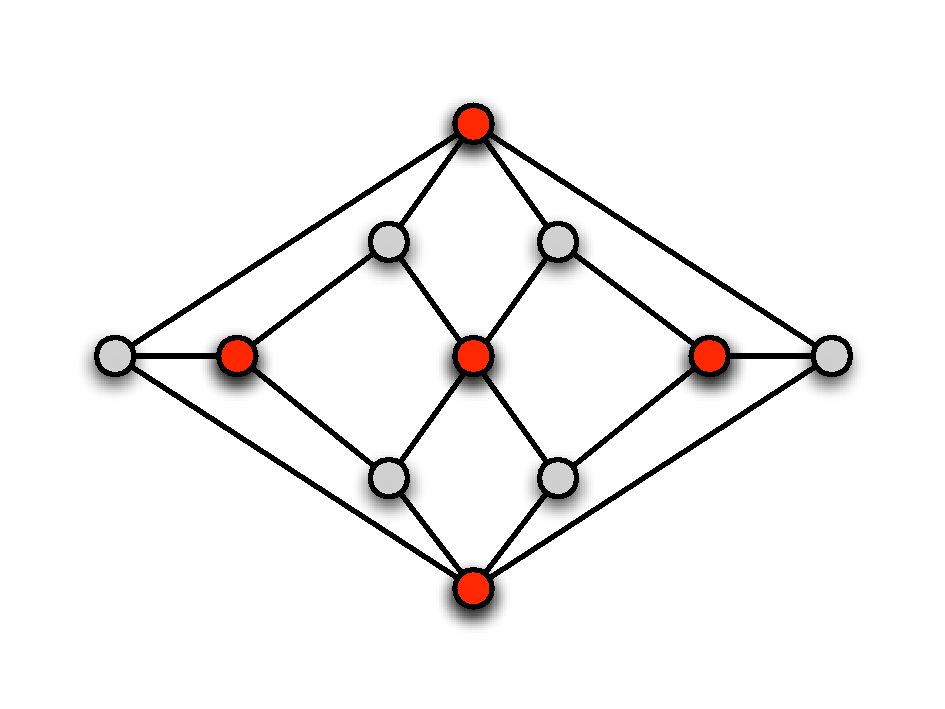
\includegraphics[width=0.6\textwidth]{pic1.pdf}
\end{center}
\caption{Herschelov graf, vektorska grafika.}
\label{pic1}
\end{figure}
Pa res lahko vključimo slike katerihkoli formatov? 
Žal ne. 
Programski paket \LaTeX\ lahko uporabljamo v več dialektih. 
Ukaz {\tt latex} ne mara vključenih slik v formatu Portable Document Format {\tt .pdf}, ukaz {\tt pdflatex} pa ne prebavi slik v Encapsulated Postscript Formatu {\tt .eps}.
Strnjeno v tabeli~\ref{tbl:1}.

\begin{table}
\begin{center}
\begin{tabular}{l|ccc}
ukaz/format & {\tt .pdf} & {\tt .eps} & ostali formati \\ \hline
{\tt pdflatex} & da & ne & da \\
{\tt latex}   & ne & da  & da
\end{tabular}
\end{center}
\caption{}
\label{tbl:1}
\end{table}

Nasvet? 
Odločite se za uporabo ukaza {\tt pdflatex}. Vaš izdelek bo brez vmesnih stopenj na voljo v {.pdf} formatu in ga lahko odnesete v vsako tiskarno. 
Če morate na vsak način vključiti sliko, ki jo imate v {\tt .eps} formatu, jo vnaprej pretvorite v alternativni format, denimo {\tt .pdf}.

Včasih se da v okolju za uporabo programskega paketa \LaTeX\ nastaviti na kakšen način bomo prebavljali vhodne dokumente. 
Spustni meni na Sliki~\ref{pic2} odkriva uporabo \LaTeX{}a v njegovi pdf inkarnaciji --- {\tt pdflatex}.
\begin{figure}[t]
\begin{center}

\includegraphics[width=10cm]{pic2.png}
\end{center}
\caption{Kateri dialekt uporabljati?}
\label{pic2}
\end{figure}
Vključena Slika~\ref{pic2} je seveda bitna.

Na vse slike in tabele se moramo v besedilu tudi sklicevati, saj kot plovke v oblikovanem besedilo niso nujno na istem mestu kot v izvornem besedilu.


\subsection{Podnapisi k slikam in tabelam}

Vsaki sliki ali tabeli moramo dodati podnapis, ki na kratko pojasnuje, kaj je na sliki ali tabeli. 
Če nekdo le prelista diplomsko delo, naj bi že iz slik in njihovih podnapisov lahko na grobo razbral, kakšno temo naloga obravnava.

Če slike povzamemo iz drugih virov, potem se moramo v podnapisu k taki sliki sklicevati na ta vir!


\chapter{Struktura strokovnih besedil}
\label{stroka}

Strokovna besedila imajo ustaljeno strukturo, da bi lahko hitreje in lažje brali in predvsem razumeli taka besedila, saj načeloma vemo vnaprej, 
kje v besedilu se naj bi nahajale določene informacije.

Najbolj osnove sestavine strokovnega besedila so:
\begin{description}
\item[naslov besedila,] ki naj bo sicer kratek, a kljub temu dovolj poveden o vsebini besedila,
\item[imena avtorjev] so običajno navedena po teži prispevka, prvi avtor je tisti, ki je besedilo dejansko pisal, zadnji pa tisti, ki je raziskavo vodil,
\item[kontaktni podatki] -- poleg imena in naslova institucije je potreben vsaj naslov elektronske pošte,
\item[povzetek] je kratko besedilo, ki povsem samostojno povzame vsebino in izpostavi predvsem  glavne rezultate ali zaključke,
\item[ključne besede] so tudi namenjene iskanju vsebin med množico člankov,
\item[uvodno poglavje] uvede bralca v tematiko besedila, razloži kaj je namen besedila, predstavi področje o katerem besedilo piše 
(če temu ni namenjeno v celoti posebno poglavje) ter na kratko predstavi strukturo celotnega besedila,
\item[poglavja] tvorijo zaokrožene celote, ki se po potrebi še nadalje členijo na podpoglavja, namenjena so recimo opisu orodij, 
ki smo jih uporabili pri delu, teoretičnim rezultatom ali predstavitvi rezultatov, ki smo jih dosegli,
\item[zaključek] še enkrat izpostavi glavne rezultate ali ugotovitve, jih primerja z dosedanjimi in morebiti poda tudi ideje za nadaljne delo,
\item[literatura] je seznam vseh virov, na katere smo se pri svojem delu opirali, oziroma smo se na njih sklicevali v svojem besedilu.
\end{description}

Strokovna besedila običajno pišemo v prvi osebi množine, v nevtralnem in umirjenem tonu. 
Uporaba sopomenk ni zaželjena, saj želimo zaradi lažjega razumevanja za iste pojme vseskozi uporabljati iste besede.
Najpomenbnejše ugotovitve je smiselno večkrat zapisati, na primer v povzetku, uvodu, glavnem delu in zaključku.
Vse trditve naj bi temeljile bodisi na lastnih ugotovitvah (izpeljavah, preizkusih, testiranjih) ali pa z navajanjem ustreznih virov.

Največ se lahko naučimo s skrbnim branjem dobrih zgledov takih besedil.


\chapter{Pogoste napake pri pisanju v slovenščini}  % poglavje dodal Solina
\label{slo}

V slovenščini moramo paziti  pri uporabi pridevnikov, ki se ne sklanjajo kot so npr. kratice. 
Pravilno pišemo model CAD in \textbf{ne} CAD model!

Pri sklanjanju tujih imen ne uporabljamo vezajev, pravilno je Applov operacijski sistem in \textbf{ne} Apple-ov.

Pika, klicaj in vprašaj so levostični: pred njimi ni presledka, za njimi pa. 
Klicajev in vprašajev se v strokovnih besedilih načeloma izogibamo. Oklepaji so desnostični in zaklepaji levostični (takole).

V slovenščini pišemo narekovaje drugače kot v angleščini!   
Običajno uporabljamo dvojne spodnje-zgornje narekovaje:  \sn{slovenski narekovaji}.
Za slovenske narekovaje je v tej predlogi definiran nov ukaz \verb+ \sn{ ... }+.

Vezaj  je levo in desno stičen: \verb=slovensko-angleški slovar= in ga pišemo z enim pomišljajem.

V slovenščini je pred in po pomišljaju presledek, ki ga v LaTeXu pišemo z dvema pomišljajema: \verb=Pozor -- hud pes!=
V angleščini pa je za razliko pomišljaj levo in desno stičen in se v LaTeXu piše s tremi  pomišljaji: \verb=---=.
S stičnim pomišljajem pa lahko nadomeščamo predlog od \dots do, denimo pri navajanju strani, npr. preberite strani 7--11 (\verb=7--11=).



\sn{Pred ki, ko, ker, da, če vejica skače}. To osnovnošolsko pravilo smo v življenju po potrebi uporabljali, dopolnili, morda celo pozabili. 
Pravilo sicer drži, ampak samo če je izpolnjenih kar nekaj pogojev (npr. da so ti vezniki samostojni, enobesedni, ne gre za vrivek itd.).
Povedki so med seboj ločeni z vejicami, razen če so zvezani z in, pa, ter, ne–ne, niti–niti, ali, bodisi, oziroma.
Sicer pa je bolje pisati kratke stavke kot pretirano dolge.

V računalništvu se stalno pojavljajo novi pojmi in nove besede, za katere pogosto še ne obstajajo uveljavljeni slovenski izrazi.
Kadar smo v dvomih, kateri slovenski izraz je primeren, si lahko pomagamo z Računalniškim slovarčkom~\cite{slovarcek}.





\chapter{Koristni nasveti pri pisanju v \LaTeX{u}}   % poglavje dodal Solina
\label{latex}

Programski paket \LaTeX\ je bil prvotno predstavljen v priročniku~\cite{lamport} in je v resnici nadgradnja sistema \TeX\ avtorja Donalda Knutha~\cite{knuth}, 
znanega po svojih knjigah o umetnosti programiranja, 
ter Knuth-Bendixovem algoritmu~\cite{knuth1983simple}.

Različnih implementacij \LaTeX{}a je cela vrsta.
Za OS X priporočamo TeXShop, za Windows PC pa MikTeX. Spletna verzija, ki poenostavi sodelovanje pri pisanju, je npr. ShareLaTeX.

Včasih smo si pri pisanju v \LaTeX{}u  pomagali predvsem s tiskanimi pri\-ro\-čni\-ki, danes pa je enostavneje in hitreje, da ob vsakem problemu za pomoč enostavno povprašamo Google, 
saj je na spletu cela vrsta forumov za pomoč pri \TeX{}iranju.

\LaTeX\ včasih ne zna deliti slovenskih besed, ki vsebujejo črke s strešicami. 
Če taka beseda štrli preko desnega roba,  \LaTeX{}u pokažemo, kje lahko tako besedo deli, takole: \verb=ra\-ču\-nal\-ni\-štvo=.
Katere vrstice štrlijo preko desnega roba, se lahko prepričamo tako, da dokument prevedemo s vključeno opcijo \texttt{draft}: \verb=\documentclass[a4paper, 12pt, draft]{book}=.


Predlagamo, da v izvornem besedilu začenjate vsak stavek v novi vrstici, saj \LaTeX\ sam razporeja besede po vrsticah postavljenega besedila. 
Bo pa zato iskanje po izvornem besedilu in popravljanje veliko hitrejše. 
Večina sistemov za \TeX{}iranje sicer omogoča s klikanjem enostavno preklapljanje  iz prevedenega besedila na ustrezno mesto v izvornem besedilu in obratno.

Boljšo preglednost dosežemo, tako kot pri pisanju programske kode, tudi z izpuščanjem praznih vrstic za boljšo preglednost strukture izvornega besedila.

S pomočjo  okolja \verb=\begin{comment} ... \end{comment}= lahko  hkrati zakomentiramo več vrstic izvornega besedila.

Pri spreminjanju in dodajanju izvornega besedila je najbolje pogosto prevajati, da se sproti prepričamo, če so naši nameni izpolnjeni pravilno.

Kadar besedilo, ki je že bilo napisano z nekim vizualnim urejevalnikom (npr. z Wordom), želimo prenesti v \LaTeX, je tudi najbolje to delati postopoma s posameznimi bloki besedila, 
tako da lahko morebitne napake hitro identificiramo in odpravimo.
Za prevajanje Wordovih datotek v \LaTeX\ sicer obstajajo prevajalniki, ki pa običajno ne generirajo take čiste logične strukture besedila, kot jo  \LaTeX\ omogoča.
Hiter in enostaven način prevedbe besedila, ki  zahteva sicer ročne dopolnitve, poteka tako, da besedilo urejeno z vizualnim urejevalnikom najprej shranimo v formatu pdf, 
nato pa to besedilo uvozimo v urejevalnik, kjer urejamo izvorno besedilo v formatu \LaTeX.


\section{Pisave v \LaTeX u}

V  \LaTeX ovem okolju lahko načeloma uporabljamo poljubne pisave. 
Izbira poljubne pisave pa ni tako enostavna kot v vizualnih urejevalnikih besedil.
Posamezne oblikovno medseboj usklajene pisave so običajno združene v družine pisav.
V \LaTeX u se privzeta družina pisav imenuje Computer Modern,
kjer so poleg navadnih črk (roman v \LaTeX u) na voljo tudi kurzivne črke (\textit{italic} v \LaTeX u), 
krepke (\textbf{bold} v \LaTeX u), kapitelke (\textsc{small caps} v \LaTeX u), linearne črke ({\textsf{san serif} v \LaTeX u),                                                                                                                                                                                                                                                                                                                           
in druge pisave.
V istem dokumentu zaradi skladnega izleda uporabljamo običajno le pisave ene družine. 

Ko začenjamo uporabljati \LaTeX, je zato najbolj smiselno uporabljati kar privzete pisave, s katerimi je napisan tudi ta dokument.
Z ustreznimi ukazi  lahko nato preklapljamo med navadnimi, kurzivnimi, krepkimi in drugimi pisavami. 
Zelo enostavna je tudi izbira velikosti črk.
\LaTeX\  odlično podpira večjezičnost, tudi v sklopu istega dokumenta, saj obstajajo pisave za praktično vse jezike, tudi take, ki ne uporabljajo latinskih črk.

Za prikaz programske kode se pogosto uporablja pisava, kjer imajo vse črke enako širino, kot so bile nekdaj črke na pisalnem stroju ({\texttt{typewriter} v \LaTeX u).

Najbolj priročno okolje za pisanje kratkih izsekov programske kode je okolje \texttt{verbatim}, saj ta ohranja vizualno organizacijo izvornega besedila in ima privzeto pisavo pisalnega stroja.

\begin{verbatim}
for (i = 0; i < 100; i++)
   for (j = i; j < 10; j++)
      some_function(i, j);
\end{verbatim}


\chapter{Kaj pa literatura?}
\label{lit}

Kot smo omenili že v uvodu, je pravi način za citiranje literature uporaba \BibTeX{}a~\cite{bib}. 
\BibTeX\ zagotovi, da nobene obvezne informacije pri določeni vrsti literature ne izpustimo in da vse informacije o določeni vrsti vira dosledno navajamo na enak način.

Osnovna ideja \BibTeX{a} je, da vse informacije o literaturi zapisujete v posebno datoteko, v našem primeru je to \texttt{literatura.bib}.
Vsakemu viru v tej datoteki določimo simbolično ime.
V  našem primeru je v tej datoteki nekaj najbolj značilnih zvrsti literature, kot so knjige~\cite{lamport}, 
članki v revijah~\cite{leonardo} in zbornikih konferenc~\cite{poglavje_springer}, 
spletni viri~\cite{bib,slovarcek,video}, 
tehnično poročilo~\cite{andersen2012kinect}, 
diplome~\cite{diploma} itd.
Diploma~\cite{diploma} iz leta 1990 je bila prva diploma na Fakulteti za elektrotehniko in računalništvo, ki je bila oblikovana z \LaTeX om!

Po vsaki spremembi pri sklicu na literaturo moramo najprej prevesti izvorno besedilo s prevajalnikom \LaTeX, nato s prevajalnikom  \BibTeX, ki ustvari datoteko  {\tt vzorec\_dip\_Seminar.bbl}, in nato še dvakrat s prevajalnikom  \LaTeX.

Kako natančno se spisek literature nato izpiše (ali po vrstnem redu sklicevanja, ali po abecedi priimkov prvih avtorjev, ali se imena avtorjev pišejo pred priimki itd.) je odvisno od stilske datoteke.
V diplomi bomo uporabili osnovno stilsko datoteko \texttt{plain}, ki vire razporedi po abecedi.
Zato je potrebno pri določenih zvrsteh literature, ki nima avtorjev, dodati polje \texttt{key}, ki določi vrstni red vira po abecedi.

Z uporabo \BibTeX{a} v slovenščini je še nekaj nedoslednosti, saj so pomožne besede, ki jih \BibTeX\ sam doda,  kot so \textit{editor},  \textit{pages} in besedica  \textit{and} pred zadnjim avtorjem, 
če ima vir več avtorjev~\cite{andersen2012kinect}, zapisane v angleščini,
čeprav smo izbrali opcijo \texttt{slovene} pri paketu \texttt{babel}.
To nedoslednost je možno popraviti z ročnim urejanjem datoteke {\tt vzorec\_dip\_Seminar.bbl}, 
kar pa je smiselno šele potem, ko bibliografije v datoteki \texttt{literatura.bib} ne bomo več spreminjali,
oziroma ne bomo več dodajali novih sklicev na literaturo v izvornem besedilu.
Vsebino datoteke {\tt vzorec\_dip\_Seminar.bbl} lahko na koncu urejanja tudi vključimo kar v izvorno besedilo diplome, tako da je vso besedilo, vključno z literaturo, zajeto le v eni datoteki.

Ko začenjamo uporabljati \BibTeX\ je lažje, če za urejanje datoteke .bib uporabljamo kar isti urejevalnik kot za urejanje datotek .tex, 
čeprav obstajajo tudi posebni urejevalniki oziroma programi za delo z \BibTeX om.

Le če se bomo na določen vir v besedilu tudi sklicevali, se bo pojavil tudi v spisku literature.
Tako je avtomatično zagotovljeno, da se na vsak vir v seznamu literature tudi sklicujemo v besedilu diplome.
V datoteki \texttt{.bib} imamo sicer lahko veliko več virov za literaturo, kot jih bomo uporabili v diplomi.

Vire v formatu \BibTeX\ lahko enostavno poiščemo in prekopiramo iz akademskih portalov za iskanje znanstvene literature v našo datoteko \texttt{.bib}, na primer v Google učenjaku.
Izvoz v Google učenjaku še dodatno poenostavimo, če v nastavitvah izberemo \BibTeX\ kot želeni format za izvoz navedb.
Navedbe, ki jih na tak način prekopiramo, pa moramo pred uporabo vseeno preveriti, saj so taki navedki običajno generirani povsem avtomatično.

Pri sklicevanju na literaturo na koncu stavka pazite, da je pika po ukazu \verb=\cite{ }=.
Da \LaTeX\ ne bi delil vrstico ravno tako, da bi sklic na literaturo v oglatih oklepajih začel novo vrstico, lahko pred sklicem na literaturo dodamo nedeljiv presledek: \verb=~\cite{ }=.


\section{Izbiranje virov za spisek literature}

Dandanes  se skoraj  vsi pri iskanju informacij vedno najprej lotimo iskanja preko svetovnega spleta.
Rezultati takega iskanja pa so pogosto spletne strani, ki danes obstajajo, jutri pa jih morda ne bo več, ali pa vsaj ne v taki obliki, kot smo jo prebrali.
Smisel navajanja literature pa je, da tudi po dolgih letih nekdo, ki bo bral vašo diplomo, lahko poišče vire, ki jih navajate v diplomi.
Taki viri pa so predvsem članki v znanstvenih revijah, ki se arhivirajo v knjižnicah, založniki teh revij pa večinoma omogočajo tudi elektronski dostop do arhiva vseh njihovih člankov.

Znanstveni rezultati, ki so objavljeni v obliki recenziranih člankov, bodisi v konferenčnih zbornikih, še bolje pa v znanstvenih revijah, so veliko bolj izčiščen in zanesljiv vir informacij, saj
so taki članki šli skozi recenzijski postopek.
Zato na svetovnem spletu začenjamo iskati vire za strokovna besedila predvsem preko akademskih spletnih portalov, kot so npr. Google učenjak, Research Gate ali Academia, saj
 so tam rezultati iskanja akademske publikacije.
Če je za dostop do nekega članka potrebno plačati, se obrnemo za pomoč in dodatne informacije na  našo knjižnico.

Če res ne gre drugače, pa je pomembno, da pri sklicevanju na spletni vir, vedno navedemo tudi datum, kdaj smo dostopali do tega vira.



\chapter{Sistem STUDIS in PDF/A}
\label{PDF}

Elektronsko verzijo diplome moramo oddati preko sistema STUDIS v formatu PDF/A ~\cite{pdfa}.
Natančneje v formatu PDF/A-1b. 

\LaTeX\ in omenjeni format imata še nekaj težav s sobivanjem. 
Paket \texttt{pdfx.sty}, ki naj bi \LaTeX{u} omogočal podporo formatu PDF/A ne deluje v skladu s pričakovanji. 
Ta predloga delno ustreza formatu, vsekakor dovolj, da jo študentski informacijski sistem sprejme. 
Znaten del rešitve je prispeval Damjan Cvetan.

V predlogi, poleg izvornega  dokumenta \texttt{.tex} in vloženih slik \texttt{pic1.pdf} in \texttt{pic2.png}, 
potrebujemo še predlogo datoteke z metapodatki \texttt{pdfa-1b.xmp} in datoteko z barvnim profilom \texttt{sRGBIEC1966-2.1.icm}.




\chapter{Sklepne ugotovitve}

Uporaba \LaTeX{a} in \BibTeX{a} je v okviru Diplomskega seminarja \textbf{obvezna}!
Izbira \LaTeX\ ali ne \LaTeX\ pri pisanju dejanske diplomske naloge pa je pre\-pu\-šče\-na dogovoru med vami in vašim mentorjem.

Res je, da so prvi koraki v \LaTeX{}u težavni. 
Ta dokument naj vam služi kot začetna opora pri hoji.
Pri kakršnihkoli nadaljnih vprašanjih ali napakah pa svetujem uporabo Googla, saj je spletnih strani za pomoč pri odpravljanju težav pri uporabi \LaTeX{}a ogromno.


\newpage %dodaj po potrebi, da bo številka strani za Literaturo v Kazalu pravilna!
\ \\
\clearpage
\addcontentsline{toc}{chapter}{Literatura}
\bibliographystyle{plain}
\bibliography{literatura}


\end{document}

